\section{Proposed Methodology}
\label{sec:4_first_proposed_approach}

This section outlines the primary phases of the study, comprising three distinct stages. Following this introduction, the synthetic data-generator method is explored in detail, offering a comprehensive breakdown of the four essential steps. Our proposal aims to develop a robust approach designed to overcome the challenging domain of multiclass classification for imbalanced and drifting data streams. To achieve this objective, the proposed solution tackles the four primary challenges associated with developing this approach.
\begin{itemize}
	\item \textbf{Multi-class imbalanced streams:} This study focuses on addressing the widespread problem of imbalanced data streams in the context of multiple classes, aiming to tackle this issue using well-known techniques, particularly MLSMOTE and MLSOL.
	\item \textbf{Overlapping class:} A critical challenge involving class overlapping, which is known to substantially affect model performance \cite{cruz2017meta, widmer1996learning}, is also addressed. An adaptive method is introduced to generate non-overlapping synthetic instances, thereby enhancing the overall performance of the model.
	\item \textbf{Drifted streams:} First proposed approach integrates a concept drift detector to identify shifts in the underlying data distribution. This dynamic detection mechanism enables the model to promptly recognize changes and adjust its classifiers, thereby ensuring its effectiveness in handling drifting stream.
	\item \textbf{Classifier performance:} To enhance the classifier performance, tfirst approach employs Dynamic Ensemble Selection (DES). This technique creates a pool of classifiers and dynamically selects the most suitable classifier for each incoming data point, further improving classification performance and robustness.
\end{itemize}

\subsection{First Proposed Approach (PA1) Description}

First proposed approach is designed with three distinct phases that work together to improve its performance in managing multiclass imbalanced and drifting data streams. 
\begin{itemize}
	\item \textbf{DES phase (dynamic ensemble selection phase):} The first phase, known as the dynamic ensemble selection (DES) phase, is responsible for selecting the most appropriate classifier for the incoming data. This ensures that the selected classifier is well-suited for the current data chunk.
	\item \textbf{Drift detector phase:} The second phase of the first approach is the drift detector phase, which operates in real-time to continuously monitor the data stream. Its primary function is to identify any signs of concept drift, which indicates shifts in the underlying data distribution over time.
	\item \textbf{Synthetic data generator phase:} The final phase of the first approach is the synthetic data generator phase, which is dedicated to generating synthetic data for the minority classes. This step is crucial for addressing class imbalance by producing additional samples for underrepresented classes, thereby significantly enhancing the model's ability to accurately classify instances from minority classes.
	\item \textbf{Synthetic data generator phase:} The final phase of the first approach is the synthetic data generator phase, which is dedicated to generating synthetic data for the minority classes. This step is crucial for addressing class imbalance by producing additional samples for underrepresented classes, thereby significantly enhancing the model's ability to accurately classify instances from minority classes.
\end{itemize}
\begin{figure}[H]
	\centering
	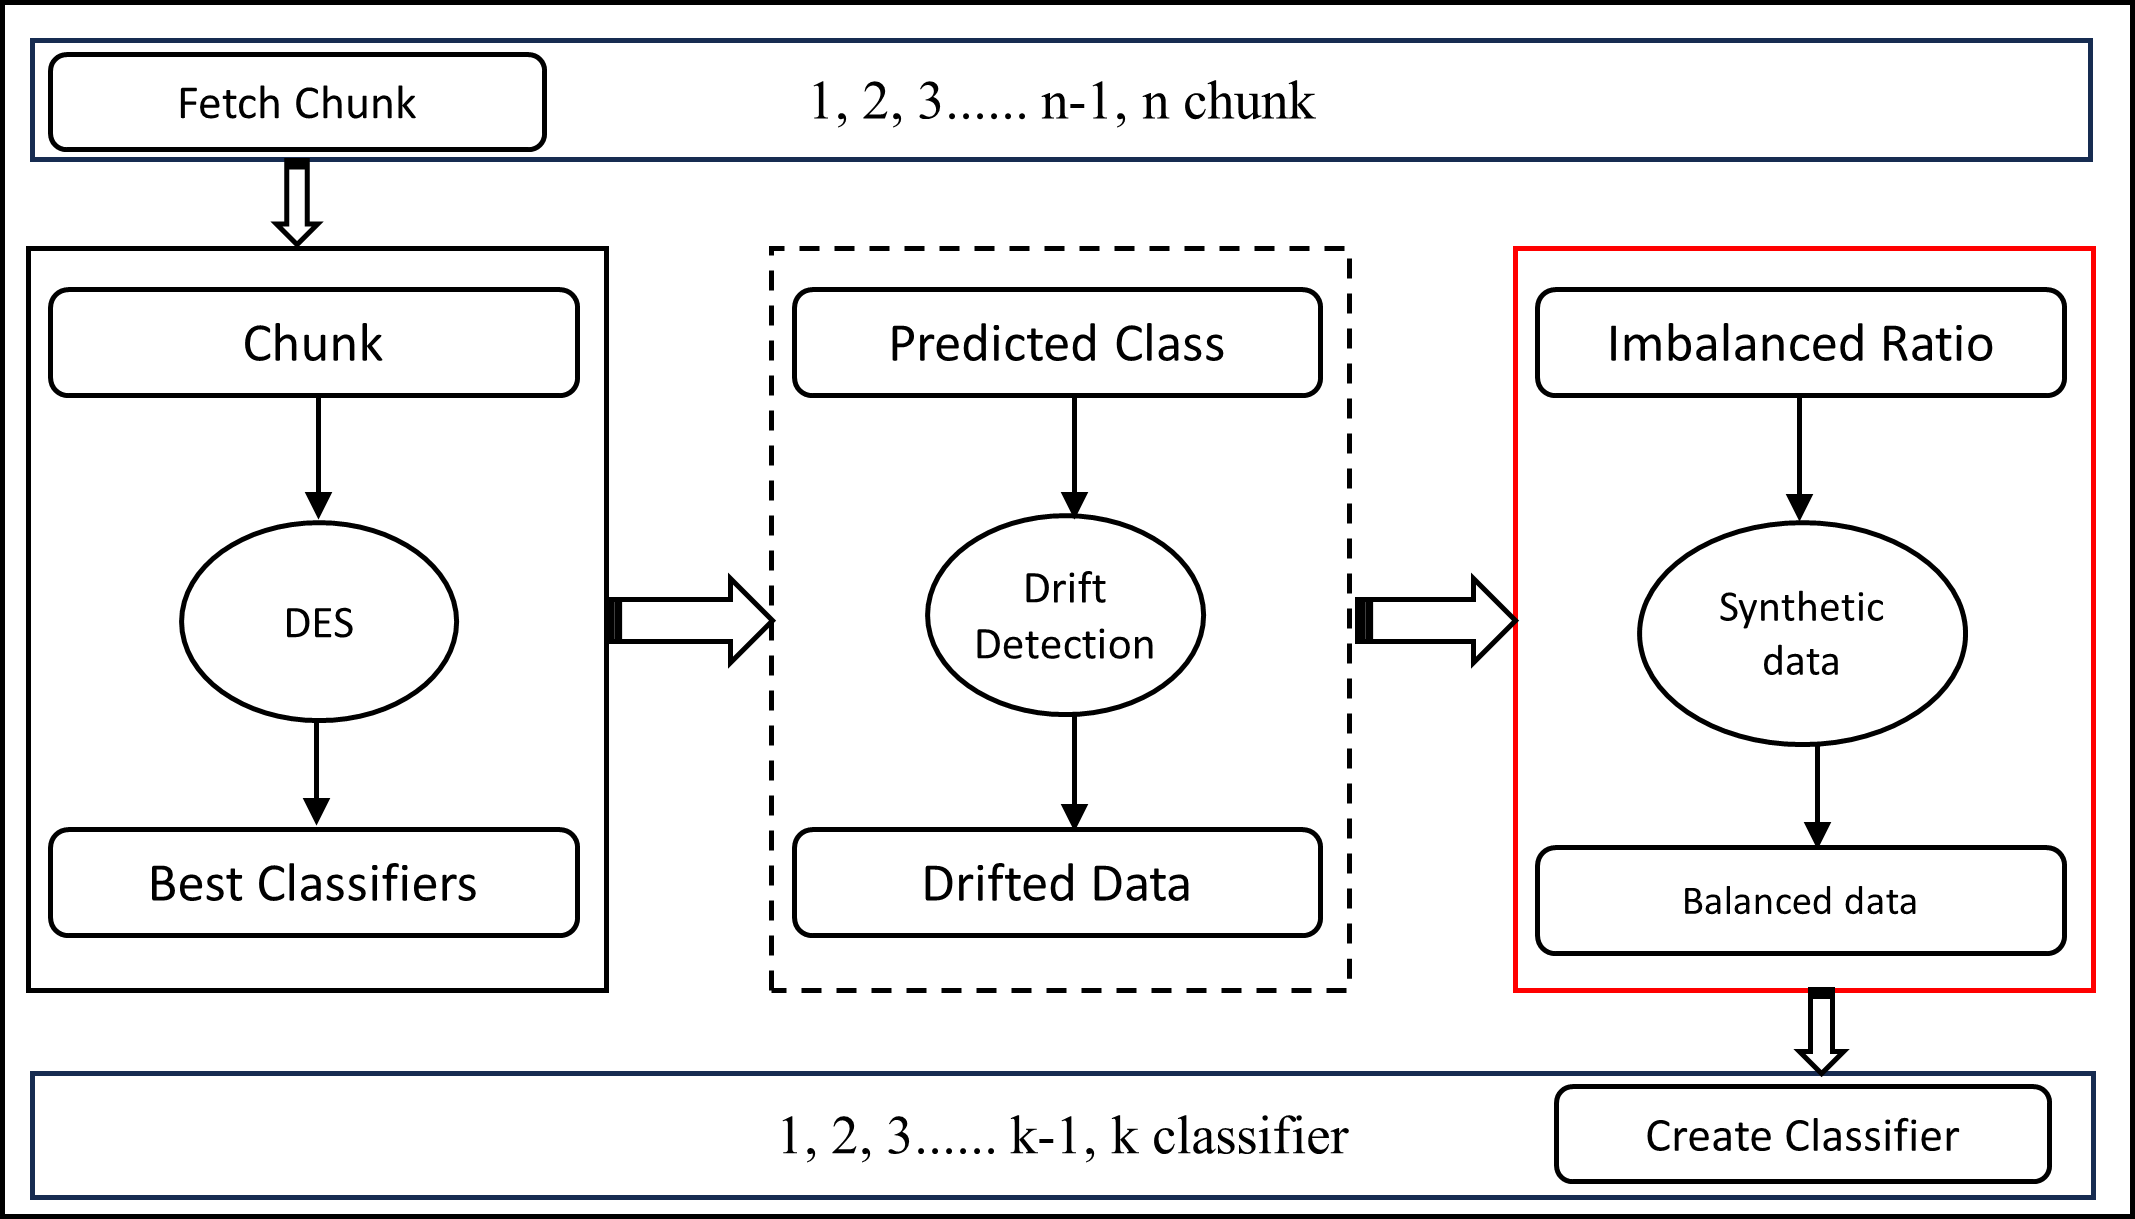
\includegraphics[width=1\linewidth]{4_Imbalanced/figures/approach_step_1.png}
	\caption{First Proposed Approach (PA1) for Imbalanced Multi-class Drifted Streams.}
	\label{fig:4_first_proposal_step_1}
\end{figure}
Specifically, as shown in Fig. \ref{fig:4_first_proposal_step_1}, the DES phase retrieves the current data chunk from the stream and applies the DES technique to select the most suitable classifiers for the received chunk. The selected classifiers were then passed to the second phase, where they were employed to predict the class of each instance within the received data chunk. Simultaneously, detectors like ADWIND or DDM are employed to monitor any occurrence of concept drift. If the discrepancy between the class frequency and standard deviation of the current chunk is significant, as described in reference \cite{gama2004learning}, and the imbalance ratio exceeds the average imbalance ratio, the current chunk is forwarded to the third phase, as indicated by the red rectangle in Fig. \ref{fig:4_first_proposal_step_1}. In the third phase, first proposed method uses a set of equations \ref{eq:4_first_proposal_1}\ref{eq:4_first_proposal_2}\ref{eq:4_first_proposal_3}
to identify minority classes. The initial equation computes the frequency of each class within the current chunk, where $i$ represents the current chunk, $c$ denotes the input class, and $y_i$ refers to the predicted class. The second equation determines the optimal frequency for each class based on the size of the chunk ($n$) and the number of classes in the current chunk($C$).

\begin{algorithm}[H]
	\caption{First Proposed Approach for Imbalanced Multi-class Streams.}
	\label{alg:4_alg_1}
	\KwIn{data stream, maximum classifiers pool size $\kappa$}
	\KwOut{Prediction $P$}
	\BlankLine
	$\psi, \Psi, \Omega, \mu \gets \emptyset$\;
	$\omega \gets 0$\;
	\For{stream have chunk}{
		\eIf{$a$ is the First chunk}{
			$k \gets$ \texttt{trainingNewClassifier}($a$)\;
			$P \gets$ \texttt{getPrediction}($a, k$)\;
		}{
			$k \gets$ \texttt{DES}($a, \Psi$)\;
			$P \gets$ \texttt{getPrediction}($a, k$)\;
			$\psi \gets$ \texttt{conceptDriftDetector}($P$)\;
			\If{$\psi > 0$}{
				$\Omega \gets$ get classes frequency according to Eq.1\;
				$\omega \gets$ best frequency according to Eq.2\;
				$\mu \gets$ get minority classes according to Eq.3\;
				$b \gets$ utilize $a$ and $\mu$ to get the synthetic data according to Algorithm \ref{alg:4_alg_2}\;
				trainingData $\gets a + b$\;
				$k \gets$ \texttt{trainingNewClassifier}(trainingData)\;
				$\Psi \gets \Psi + k$\;
				\If{$\Psi > \kappa$}{
					\texttt{removeWorstClassifier}($\Omega$)\;
				}
			}
			$P \gets$ \texttt{getPrediction}($a, k$)\;
		}
	}
	\Return{$P$}
	\end{algorithm}

Finally, the third equation identifies the classes as minority classes if their frequency deviates significantly from the standard deviation of the current chunk, where $sd_c$ represents the standard deviation of the class instances, and $frq_i$ refers to the standard deviation of the current chunk.
Figure \ref{fig:4_first_proposal_step_2} shows that phase These identified minority classes are then fed into the synthetic data generator phase, which increases the minority class samples to balance any imbalanced chunks. This ensures optimal performance for the new classifiers. Algorithm  \ref{alg:4_alg_1} provides a comprehensive outline of the process of the first proposed approach, which is the main contribution of this study and is designed to effectively address multiclass imbalanced and drifting data streams, uses streaming data as input, and systematically executes each step within the approach. The outcome of this process is the classification prediction generated using the first proposed approach.

\subsection{Synthetic Data Generator Phase Description}

Figure \ref{fig:4_first_proposal_step_2} presents a comprehensive overview of the synthetic data generator phase, which is an essential component responsible for generating synthetic samples by considering both data distribution and historical chunk behaviors. This phase has several advantages and can perform a wide range of tasks.
\begin{figure}[H]
	\centering
	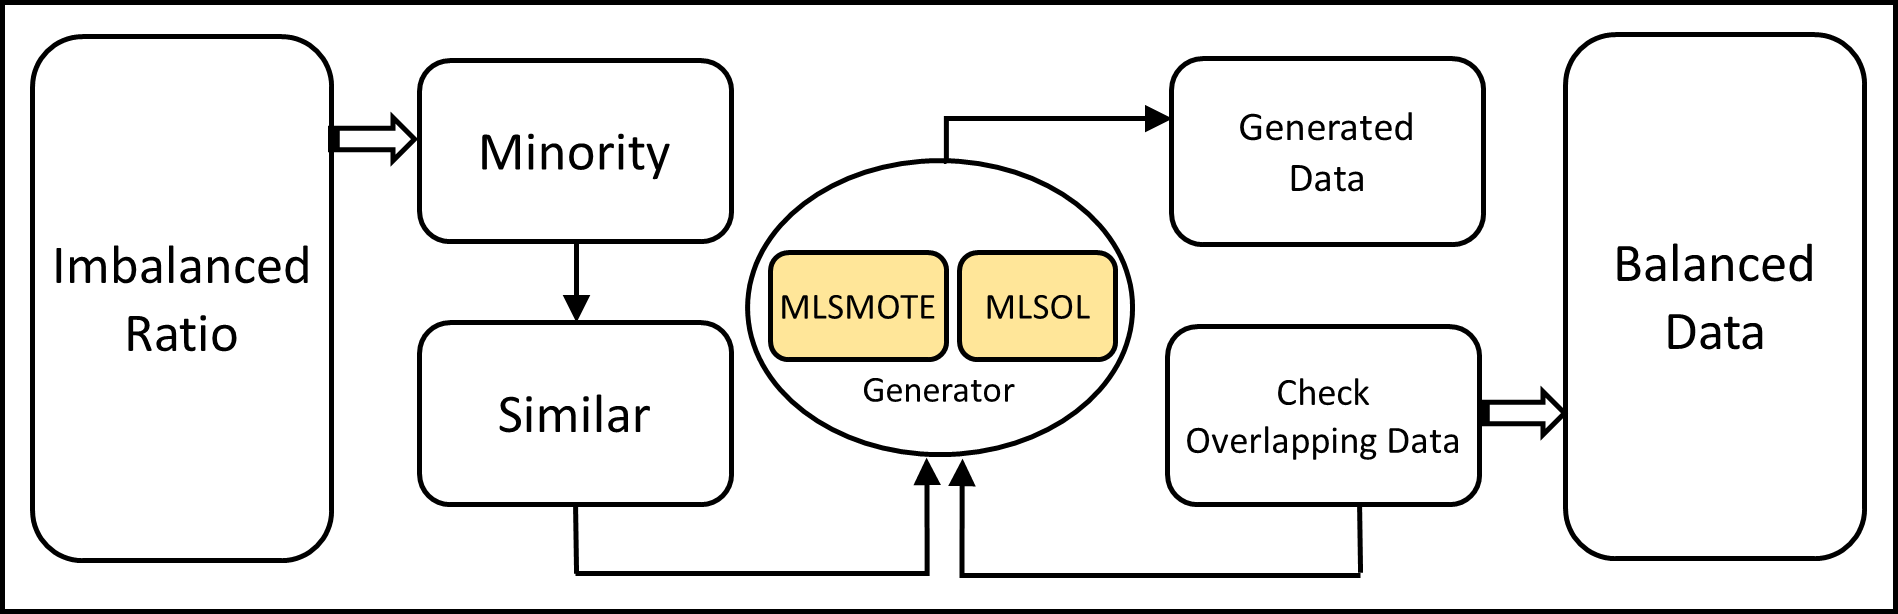
\includegraphics[width=1\linewidth]{4_Imbalanced/figures/approach_step_2.png}
	\caption{Flow Diagram of the Synthetic Data Generator.}
	\label{fig:4_first_proposal_step_2}
\end{figure}
\begin{itemize}
	\item \textbf{Similar chunk analysis:} Initially, the phase analyzes the current chunk distribution and identifies a similar chunk from historical data. This analysis forms the basis for generating synthetic samples that align with prevailing distribution patterns.
	\item \textbf{Oversampling method selection:} This phase utilizes the knowledge of the oversampling technique applied to the identified similar chunk. Consequently, it employs an alternative oversampling technique, using MLSMOTE and MLSOL, to create the most effective synthetic data. This step is designed not only to optimize the current classification but also to preemptively address potential drifts in similar future chunks.
	\item \textbf{Class overlap validation:} This step involves generating synthetic samples for the minority classes to effectively address the issue of minority classes and consequently enhance the classifier performance. The process utilizes the K-Nearest Neighbor (KNN) algorithm, as applied in \cite{lu2016concept}, to identify overlaps between newly generated data instances and existing instances. If overlaps are detected, the first proposed approach iteratively removes these samples because their presence can potentially diminish the overall classifier performance \cite{cruz2017meta, widmer1996learning}. Consequently, the first proposed approach generates alternative samples to address this challenge and preserve the primary objectives of the synthetic data generator step.
	\item \textbf{Continuous refinement:} This process iterates until it successfully generates high-quality synthetic data that aligns with the data distribution, minimizes overlap, and mitigates potential concept drift. The generated data were subsequently utilized in the training phase to improve classifier performance.
\end{itemize}
\begin{algorithm}[H]
	\caption{Synthetic Data Generator Algorithm.}
	\label{alg:4_alg_2}
	\KwIn{Minority classes $\mu$, current chunk $a$, sample size $\eta$, historical chunks $h$}
	\KwOut{Generated data $b$}
	$b \gets \emptyset$\;
	$f \gets \text{MLSMSOTE}$\;
	$knn \gets \text{kNearestNeighbor}(a)$\;
	$chunk \gets \text{similarChunk}(a, h)$\;
	$f \gets \text{similarChunkOverSamplingMethod}(chunk)$\;
	\If{$f = \text{MLSMSOTE}$}{
		$f \gets \text{MLSOL}$\;
	}
	\Else{
		$f \gets \text{MLSMSOTE}$\;
	}
	\While{$|b| < \eta$}{
		$p \gets \text{generateSyntheticPoint}(\mu, f)$\;
		$similarPointsClass \gets \text{KNN.getKneighbor}(b)$\;
		\If{$similarPointsClass = \mu$}{
			$b \gets b \cup \{p\}$\;
		}
	}
	\Return $b$\;
	\end{algorithm}
In Algorithm \ref{alg:4_alg_2}, also known as the Synthetic Data Generator, three essential elements are inputted: the minority class samples, the current data chunk, and the desired size for generating synthetic data. The primary objective of this algorithm is to produce synthetic data samples. To achieve this, the KNN algorithm is employed to identify any overlapping instances within the current chunk (Line 3). This algorithm utilizes two specific techniques, MLSMOTE \cite{gama2004learning} and MLSOL \cite{liu2017regional}. MLSMOTE was chosen for its introduction of randomness during instance generation, reducing its reliance on the local characteristics and distribution of the minority class. This randomization diminishes the likelihood of producing overlapping instances, particularly in cases where minority class instances are situated in overlapping regions. In contrast, MLSOL considers the local behavior of minority classes, resulting in synthetic points that closely resemble the minority class. This approach significantly improves the performance of the classifier (lines 4-10). Additionally, in this algorithm, specifically from lines 11 to 17, these lines are dedicated to generating synthetic instances that ensure non-overlap with existing classes. This procedure depends on the selected oversampling method and utilizes the KNN algorithm to guarantee that the generated instances do not overlap with the existing ones.


	\section{Mathematical Foundation for PA1}
	\label{sec:math_foundation_pa1}
	
	The mathematical foundation for PA1 involves key equations designed to identify and classify data chunks based on class frequencies and distributions. These equations are fundamental to analyzing imbalanced data streams effectively.
	
	Equation \ref{eq:4_first_proposal_1} calculates the frequency of a specific class \(c\) within a data chunk. For each instance \(y_i\), the frequency \(frq_{c}\) is incremented if the instance belongs to class \(c\):  
	\begin{equation}
	\label{eq:4_first_proposal_1}
	frq_{c} = \sum_{i=1}^{\text{chunk size}} 
	\begin{cases} 
	1, & \text{if } y_i = c \\
	0, & \text{otherwise}
	\end{cases}, \quad i = 1, 2, 3, \dots \text{chunk size}.
	\end{equation}
	
	Equation \ref{eq:4_first_proposal_2} defines the \textit{best frequency} for a chunk, \(freq_n\), as the proportion of instances \(n\) relative to the total number of classes \(C\):  
	\begin{equation}
	\label{eq:4_first_proposal_2}
	\text{best } freq_{n} = \frac{|n|}{|C|}.
	\end{equation}
	
	Finally, Equation \ref{eq:4_first_proposal_3} determines the type of each class in the chunk (\textit{Minority} or \textit{Majority}) by comparing the difference between the standard deviation (\(sd_c\)) and the class frequency (\(frq_i\)) against the best frequency of the chunk (\(freq_{\text{chunk}}\)):  
	\begin{equation}
	\label{eq:4_first_proposal_3}
	\text{classes type}_{\text{chunk}} = \sum_{c=1}^{C} 
	\begin{cases} 
	\text{Minority,} & \text{if } diff(sd_c - frq_i) > \text{best } freq_{\text{chunk}} \\
	\text{Majority,} & \text{otherwise}.
	\end{cases}
	\end{equation}
	
	These equations collectively enable precise identification of class types within data chunks, forming a critical component of the PA1 framework.
	
	